\documentclass{article}
\usepackage[utf8]{inputenc}

\title{Homework No.1}
\author{Osamu Katagiri-Tanaka : A01212611}
\date{\today}

% import math symbols
\usepackage{amsmath, esint}

% import continuous lists
\usepackage{enumitem}

% format margins and paper size
\usepackage{geometry}
\geometry{
	paper         = a4paper, % Change to letterpaper for US letter
	inner         = 2.5cm,   % Inner margin
	outer         = 2.5cm,   % Outer margin
	bindingoffset = 0.5cm,   % Binding offset
	top           = 1.5cm,   % Top margin
	bottom        = 1.5cm    % Bottom margin
}

% import figure handler
\usepackage{graphicx}

% import references handler
\usepackage[
    style     = ieee,         % references format style
    backend   = biber,        % choose the processing program
    natbib    = true,         % enable additional reference formats
    citestyle = numeric-comp, % enable multiple citations
    sortcites = true,         % sort references in multiple citations
    sorting   = nyt           % sort the reference table
]{biblatex}
\addbibresource{references.bib}

% Note that ‘d’ in the differential is conventionally set in roman.
\newcommand{\ud}{\,\mathrm{d}}

% Paragraph spacing
\setlength{\parskip}{0.2cm}           % spacing between paragraphs
\renewcommand{\baselinestretch}{1.25} % spacing between lines

\begin{document}

\maketitle

\section*{\emph{What will I achieve?}}
With this homework you will practice the use of the concepts and knowledge acquired throughout the corresponding topics.

\section*{Instructions}

\subsection*{Part A}
\textit{Find five differential equations found in fluid mechanics, heat transfer, mass transfer, bioengineering or reaction engineering. Three of them must be PDE (Partial differential equations), and you must explain each term, the physical meaning of each term, and what they represent.}

\subsubsection*{Conservation of Mass : Continuity Equation}

\begin{equation}
\frac{\ud}{\ud t} \iiint \rho \ud V + \oiint \vec{n} \cdot (\rho \vec{v}) \ud A = \frac{\partial \rho}{\partial t} + \vec{\nabla} \cdot (\rho \vec{v}) = 0
\label{eq_continuityEquation}
\end{equation}

For closed systems, the conservation of mass principle is achieved by fixing the mass to a constant; however for control volumes, mass can move through the boundaries. The continuity equation must monitor the amount of mass entering and leaving the control volume, see Equation \ref{fig_changeOfMass}. The conservation of mass equation \ref{eq_continuityEquation} is obtained by replacing $B$ in the Reynolds transport theorem by mass $m$, and $\hat{B}$ by 1 ($m$ per unit mass = $1$), and states that the time rate of change of mass plus the mass flow rate in the control volume is equal to zero \cite{White2011, Moukalled2016}.

\begin{equation}
\left(
    \begin{array}{c}
        \textrm{change of mass} \\
        \textrm{within the} \\
        \textrm{control volume} \\
        \Delta m_{CV}
    \end{array}
\right) = \left(
    \begin{array}{c}
        \textrm{mass entering} \\
        m_{in}
    \end{array}
\right) - \left(
    \begin{array}{c}
        \textrm{mass leaving} \\
        m_{out}
    \end{array}
\right)
\label{fig_changeOfMass}
\end{equation}

Where: $\displaystyle m_{CV} = \iiint \rho \ud V$ is the total mass within the control volume $CV$ and $\displaystyle \frac{\ud m_{CV}}{\ud t} = \frac{\ud}{\ud t} \iiint \rho \ud V$ is the rate of change of mass within $CV$. Given the mass flow of $m_{in}$ or $m_{out}$ through a differential area $\ud A$ , the mass flow rate is dependent on the fluid density $\rho$, normal velocity $\vec{v}$, and the flow area $\ud A$. The flow rate out or into $CV$ over the entire control surface is $\displaystyle \dot{m} = \oiint \vec{n} \cdot (\rho \vec{v}) \ud A$ \cite{White2011}. In other words, if $\displaystyle \frac{\ud m_{CV}}{\ud t} < 0$, $m_{in}$ shall increase with the mass flow rate to compensate the lost mass in $m_{CV}$, or increase $m_{out}$ if $\displaystyle \frac{\ud m_{CV}}{\ud t} > 0$; hence the conservation of mass.

\subsubsection*{Conservation of Mechanical Energy : Bernoulli equation}

\begin{equation}
\frac{P}{\rho} + \frac{v^2}{2} + \textsl{g} z = constant
\label{eq_bernoulliSteadyIncompressible}
\end{equation}

The Bernoulli equation is valid in inviscid regions of a steady incompressible flow where net viscous forces are negligible compared to inertial, gravitational, or pressure forces \cite{White2011}.

\begin{figure}[h!]
\centering
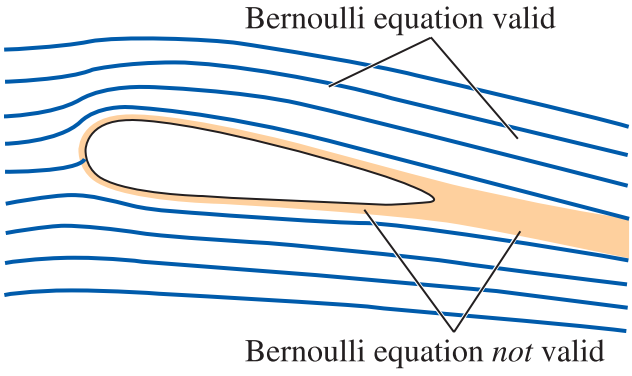
\includegraphics[width=0.45\textwidth]{./img/bermoulliInviscidRegions.png}
\caption{Adapted from \cite{White2011}}
\label{fig_bermoulliInviscidRegions}
\end{figure}

Equation \ref{eq_bernoulliSteadyIncompressible} is derived from the Bernoulli equation for a steady compressible flow $\displaystyle \int \frac{\ud P}{\rho} + \frac{v^2}{2} + \textsl{g} z = constant$, where $\rho$ is constant. Steady simply means no change in velocity $v$ with time at a specified location, but $v$ can change from one location to another. Equation \ref{eq_bernoulliSteadyIncompressible} describes a balance between pressure (flow energy) $\displaystyle \frac{P}{\rho}$, velocity (kinetic energy) $\displaystyle \frac{v^2}{2}$, and position (potential energy) $\textsl{g} z$ of fluid particles relative to the gravity vector. There are various forms of the Bernoulli equation for incompressible/compressible, steady/nonsteady, and derivations through Newton's second law (linear momentum equation) and the first law of thermodynamics. The most commonly used forms are for steady incompressible fluid flow derived through conservation of momentum, as depicted in Equation \ref{eq_bernoulliSteadyIncompressible} \cite{White2011}.

The flow, kinetic and potential energies are forms of mechanical energy, therefore the Bernoulli equation only works in systems where the mechanical energy and thermal energy are conserved separately. Equation \ref{eq_bernoulliSteadyIncompressible} states that various forms of mechanical energy are converted to each other, but their sum remains constant. There is no dissipation of mechanical energy as there is no friction that converts such mechanical energy to thermal energy. Bernoulli equation is derived from a force balance on a particle moving, hence no shaft work of considered \cite{White2011}.

\subsubsection*{Conservation of Energy : 1st Law of Thermodynamics}

\begin{equation}
\frac{\ud E}{\ud t} = \frac{\ud}{\ud t} \iiint e \rho \ud V + \oiint e \rho (\vec{v} \cdot \vec{n}) \ud A = \frac{\partial \rho e}{ \partial t} + \vec{\nabla} \cdot (\rho \vec{v} e)
\label{eq_conservationOfEnergy}
\end{equation}

The total energy within a system is affected by work transfer $W$ and heat transfer $Q$. Since energy is conserved, the total energy of the system is $\displaystyle E = Q + W$ \cite{Moukalled2016, White2011}. Unlike Bernoulli's equation, Equation \ref{eq_conservationOfEnergy} considers the heat transfer.

\textbf{Heat Transfer $Q$ :} The internal energy, heat or thermal energy tends to move from a high temperature body to a low temperature body. The temperature difference dictates the rate of heat transfer. At higher temperature differences, the higher is the rate of heat transfer. Once the temperature is balanced between the two bodies, heat transfer stops \cite{White2011}.

\textbf{Work Transfer $W$ :} Work (or mechanical energy) is an energy interaction related to a force. A system may involve several forms of work, in such a way that: $\displaystyle W = W_{motor} + W_{pressure} + W_{viscous} + \textrm{work done by other forces} \dots$. $W_{motor}$ is the work done by a rotating shaft,  $W_{pressure}$ is the work transmitted by pressure forces, and $W_{viscous}$ are the normal and shear stress components of viscous forces. $W$ can also be comprised by work done by other forces such as surface tension, magnetic and electric. $W_{viscous}$ is only considered when the moving walls are part of the control surface \cite{White2011}.

The relationship between conservation of energy for a control volume is obtained by the Reynolds transport theorem, replacing $B$ with the total energy $E$ and $\hat{B}$ with the total energy per unit mass, which is $e = \displaystyle u + \frac{v^2}{2} + \textsl{g} z = constant$. $u$, $\displaystyle \frac{v^2}{2}$, and $\textsl{g} z$ are the internal, kinetic, and potential energies per unit mass respectively \cite{Moukalled2016, White2011}. In other words, $\displaystyle \frac{\ud E}{\ud t}$ can be described as follows:

$$ \left(
    \begin{array}{c}
        \textrm{The rate of} \\
        \textrm{energy transfer by} \\
        \textrm{heat and work} \\
    \end{array}
\right) = \left(
    \begin{array}{c}
        \textrm{The time rate of} \\
        \textrm{change in energy} \\
    \end{array}
\right) + \left(
    \begin{array}{c}
        \textrm{The flow rate of} \\
        \textrm{energy out of} \\
        \textrm{the surface} \\
    \end{array}
\right) $$

\subsubsection*{Linear Momentum : Cauchy's equation}

\begin{equation}
\frac{\partial}{\partial t} (\rho \vec{v}) + \vec{\nabla} \cdot (\rho \vec{v} \vec{v}) = \rho \vec{\textsl{g}} + \vec{\nabla} \cdot \sigma_{ij}
\label{eq_cauchyEquation}
\end{equation}

Equation \ref{eq_cauchyEquation} is derived from the Reynolds transport theorem for linear momentum in a control volume ($B = m \vec{v}$ and $\hat{B} = \vec{v}$ per unit mass) \cite{White2011}. This equation states that the total force acting on the control volume is equal to the rate at which momentum changes $\displaystyle \left( \sum \vec{F}_{body} = \iiint \frac{\partial}{\partial t} (\rho \vec{v}) \ud V \right)$ plus the rate at which momentum flows out of the control volume minus the rate at which momentum flows into the control volume $\displaystyle \left( \sum_{out} \vec{F}_{surface} - \sum_{into} \vec{F}_{surface} = \oiint \vec{n} (\rho \vec{v} \vec{v}) \ud A \right)$. $\sigma_{ij}$ is the stress tensor.

Equation \ref{eq_cauchyEquation} is valid for compressible and incompressible at any point in the flow domain. However, Cauchy's equation is not able to solve any fluid mechanic problem as the stress tensor $\sigma_{ij}$ needs to be expressed in terms of unknowns such as density, pressure, velocity, viscosity, surface tension, etc \cite{White2011}.

\subsubsection*{Linear Momentun : Navier-Stokes Equation}

\begin{equation}
\rho \frac{\ud \vec{v}}{\ud t} = - \vec{\nabla} P + \rho \vec{\textsl{g}} + \mu \nabla^2 \vec{v}
\label{eq_navierStokesEquation}
\end{equation}

Equation \ref{eq_navierStokesEquation} is the Navier–Stokes equation for an incompressible flow with constant viscosity. Navier-Stokes equation is Newton's second law (conservation of momentum) adapted for a fluid particle with the viscous stress tensor $(\sigma_{ij})$ replaced by the constitutive relationship between stress $(\tau_{ij})$ and strain rate $(\varepsilon_{ij})$ tensors for Newtonian fluids as in Equation \ref{eq_vicousStressTensor} in Cartesian coordinates. In other words, Equation \ref{eq_navierStokesEquation} is the conservation of momentum for Newtonian fluids, which assumes that the viscosity $\mu$ is constant.

\begin{equation}
\begin{array}{c}
    \tau_{ij} = 2 \mu \varepsilon_{ij} \\
    \tau_{ij} = \left( 
        \begin{matrix}
            \displaystyle 2 \mu \frac{\partial u}{\partial x} &
            \displaystyle \mu \left( \frac{\partial u}{\partial y} + \frac{\partial v}{\partial x} \right) &
            \displaystyle \mu \left( \frac{\partial u}{\partial z} + \frac{\partial w}{\partial x} \right) \\
            
            \displaystyle \mu \left( \frac{\partial v}{\partial x} + \frac{\partial u}{\partial y} \right) &
            \displaystyle 2 \mu \frac{\partial v}{\partial y} &
            \displaystyle \mu \left( \frac{\partial v}{\partial z} + \frac{\partial w}{\partial y} \right) \\
            
            \displaystyle \mu \left( \frac{\partial w}{\partial x} + \frac{\partial u}{\partial z} \right) &
            \displaystyle \mu \left( \frac{\partial w}{\partial y} + \frac{\partial v}{\partial z} \right) &
            \displaystyle 2 \mu \frac{\partial w}{\partial z} \\
        \end{matrix}
    \right) \\
    \sigma_{ij} = \left( 
        \begin{matrix}
            -P &  0 &  0 \\
             0 & -P &  0 \\
             0 &  0 & -P \\
        \end{matrix}
    \right) + \tau_{ij} \\
\end{array}
\label{eq_vicousStressTensor}
\end{equation}

Notice that for a fluid at rest, the viscous stresses are neglected therefore $\tau_{ij}$ is a   `zero matrix'. Table \ref{tb_NewtonNavierStokes} relates Newton's second law $\displaystyle \sum F = m a$ with the Navier-Stokes equation.

\begin{table}[h!]
\caption{Newton's 2nd law vs. Navier-Stokes equation}
\begin{center}
\begin{tabular}{ c | c   c }
                 & Newton's 2nd law & Navier-Stokes equation \\
    \hline
    force        & $\displaystyle \sum F$ & $\displaystyle - \vec{\nabla} P + \rho \vec{\textsl{g}} + \mu \nabla^2 \vec{v}$ \\
    mass/density & $\displaystyle m$ & $\displaystyle \rho$ \\
    acceleration & $\displaystyle a$ & $\displaystyle \frac{\ud \vec{v}}{\ud t}$
\end{tabular}
\end{center}
\label{tb_NewtonNavierStokes}
\end{table}

\subsection*{\emph{Part B}}
\textit{Select one problem of any of the fields listed above, and solve it, following the steps given below.}

Problem taken from Cengel et al. \cite{Cengel2017}.

\begin{figure}[h!]
\centering
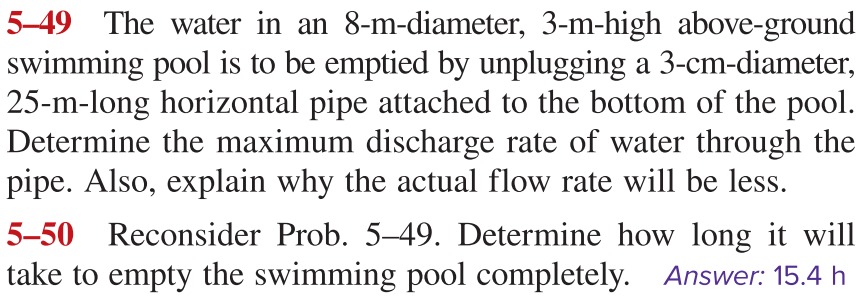
\includegraphics[width=0.60\textwidth]{./img/PROBLEMBernoulliEquation.png}
\caption{Taken from \cite{Cengel2017}}
\label{fig_PROBLEMBernoulliEquation}
\end{figure}

\begin{enumerate}
\item \textit{Read problem statement, and collect the information that may be needed.}
\end{enumerate}

\begin{itemize}
\item Cylindrical swimming pool dimensions:
    \begin{itemize}
    \item[$\circ$] $diameter = 8 m$,
    \item[$\circ$] $height = 3 m$
    \end{itemize}
\item Drainage pipe dimensions:
    \begin{itemize}
    \item[$\circ$] $diameter = 3 cm$,
    \item[$\circ$] $length = 25 m$,
    \item[$\circ$] attached at the bottom of the pool
    \end{itemize}
\end{itemize}

\begin{enumerate}[resume]
\item \textit{Make a Sketch (Diagram, process flow chart), indicating mass, linear or angular momentum (i.e. forces and torques) and energy interaction, and label each stream and boundaries as well.}
\end{enumerate}

\begin{figure}[h!]
\centering
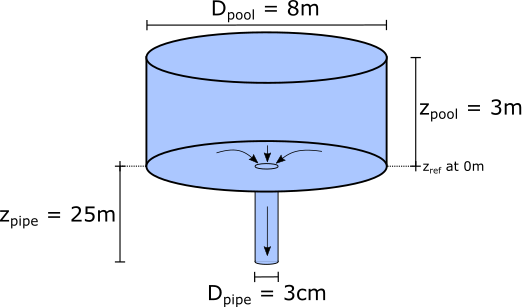
\includegraphics[width=0.70\textwidth]{./img/FIGUREBernoulliEquation.png}
\caption{Sketch}
\label{fig_FIGUREBernoulliEquation}
\end{figure}

\begin{enumerate}[resume]
\item \textit{List Assumptions and Approximations (sometimes they may be inferred by the sketch, but make them explicit) supported by equations if possible (geometric relationships, or fundamental equations).}
\end{enumerate}

\begin{itemize}
\item 
\end{itemize}

\begin{enumerate}[resume]
\item \textit{Physical Laws (Fundamental Laws) must be written in full form, and terms can be dropped by the right selection of frame of reference, operating conditions, assumptions, simplifications or constraints.}
\end{enumerate}



\begin{enumerate}[resume]
\item \textit{Physical constants should be obtained from a reliable source (knowing this information by heart is always helpful ), geometric relations and formulae must be included as part of your analysis.}
\end{enumerate}



\begin{enumerate}[resume]
\item \textit{Physical transport or thermodynamic properties (Thermodynamic relations) should be evaluated, approximated, calculated or obtained from a reliable source.}
\end{enumerate}

Not Applicable

\begin{enumerate}[resume]
\item \textit{Calculations are done including units. Any algebraic manipulation is recommended in few cases, because limits the step 8, but if needed should be done before using numerical values of constants, properties or variables.}
\end{enumerate}



\begin{enumerate}[resume]
\item \textit{Reasoning (Sensitivity analysis, what if), Verification (context), and Discussion should always be part of your answer to any problem, regardless the task requested.}
\end{enumerate}



\printbibliography[title={References}]
\end{document}